\textbf{TODO} Figure showing the different cases from the paragraph above, a and b. Give both the original circuit with dashed splits, the hypergraph and the black boxed distributed circuit (fig:vanillaCuts)
\begin{figure}
\centering
\begin{tikzpicture}
  \node (distributed) {
    \begin{tikzpicture}
      \node[inner sep=0pt] (circuit) {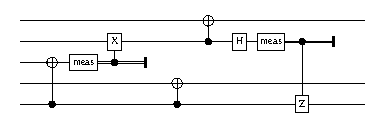
\includegraphics[scale=2]{Figures/circuits/vanillaCuts0}};
      \pic (e1) {ebit=e1/12.67mm/13mm};
      \coordinate[above left=3.6mm and -6mm of circuit.west] (leftPoint);
      \coordinate[above right=3.6mm and -6mm of circuit.east] (rightPoint);
      \pic (cut) {cut=leftPoint/rightPoint};
      \node[above left=11.5mm and -7mm of circuit.west, opacity=0.9] {\footnotesize \(A\)};
      \node[below left=4.5mm and -7mm of circuit.west, opacity=0.9] {\footnotesize \(B\)};
      \node[below left=11.5mm and -7mm of circuit.west, opacity=0.9] {\footnotesize \(C\)};
      \node[right=-3mm of circuit.north west, font=\itshape] (text) {c)};
    \end{tikzpicture}
  };
  \node[above left=-3mm and -70mm of distributed] (template) {
    \begin{tikzpicture}
      \node[inner sep=0pt] (circuit) {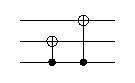
\includegraphics[scale=2]{Figures/circuits/vanillaCutsTemplate}};  
      \coordinate[above left=3.6mm and -6mm of circuit.west] (leftPoint);
      \coordinate[above right=3.6mm and -6mm of circuit.east] (rightPoint);
      \pic (cut) {cut=leftPoint/rightPoint};
      \node[above left=4.5mm and -7mm of circuit.west, opacity=0.9] {\footnotesize \(A\)};
      \node[left=-7mm of circuit.west, opacity=0.9] {\footnotesize \(B\)};
      \node[below left=4.5mm and -7mm of circuit.west, opacity=0.9] {\footnotesize \(C\)};
      \node[right=-3mm of circuit.north west, font=\itshape] (text) {a)};
    \end{tikzpicture}
  };
  \node[above right=-26.5mm and 10mm of template] (hypergraph) {
    \begin{tikzpicture}
      \coordinate (O) at (0,0);
      \coordinate (A) at (90:10mm);
      \coordinate (B) at (210:10mm);
      \coordinate (C) at (330:10mm);
      \draw (O) -- (A);
      \draw (O) -- (B);
      \draw (O) -- (C);
      \node[circle, right=-2.5mm of A, fill=white, inner sep=0pt, minimum size=5mm] {\(A\)};
      \node[circle, right=-2.5mm of B, fill=white, inner sep=0pt, minimum size=5mm] {\(B\)};
      \node[circle, right=-2.5mm of C, fill=white, inner sep=0pt, minimum size=5mm] {\(C\)};
      \coordinate[above left=5.3mm and 9mm of O] (leftPoint);
      \coordinate[above right=5.3mm and 9mm of O] (rightPoint);
      \pic (cut) {cut=leftPoint/rightPoint};
      \node[above left=0mm and 9mm of A, font=\itshape] (text) {b)};
    \end{tikzpicture}
  };
\end{tikzpicture}
\caption{The CNOTs in the circuit \textit{a)} are adjacent at their control wire. Therefore, a single hyperedge is used to represent both in \textit{b)}. The proposed cut makes only one of the CNOTs non-local, which is implemented in \textit{c)} using one ebit.}
\label{fig:vanillaCutsA}
\end{figure}

\begin{figure}
\centering
\begin{tikzpicture}
  \node (distributed) {
    \begin{tikzpicture}
      \node[inner sep=0pt] (circuit) {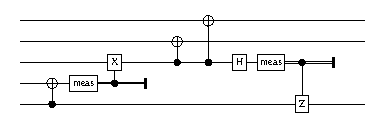
\includegraphics[scale=2]{Figures/circuits/vanillaCuts1}};
      \pic (e1) {ebit=e1/19.75mm/13mm};
      \coordinate[above left=-3.6mm and -6mm of circuit.west] (leftPoint);
      \coordinate[above right=-3.6mm and -6mm of circuit.east] (rightPoint);
      \pic (cut) {cut=leftPoint/rightPoint};
      \node[above left=11.5mm and -7mm of circuit.west, opacity=0.9] {\footnotesize \(A\)};
      \node[above left=4.5mm and -7mm of circuit.west, opacity=0.9] {\footnotesize \(B\)};
      \node[below left=11.5mm and -7mm of circuit.west, opacity=0.9] {\footnotesize \(C\)};
      \node[right=-3mm of circuit.north west, font=\itshape] (text) {c)};
    \end{tikzpicture}
  };
  \node[above left=-3mm and -70mm of distributed] (template) {
    \begin{tikzpicture}
      \node[inner sep=0pt] (circuit) {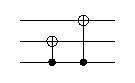
\includegraphics[scale=2]{Figures/circuits/vanillaCutsTemplate}};  
      \coordinate[below left=3.6mm and -6mm of circuit.west] (leftPoint);
      \coordinate[below right=3.6mm and -6mm of circuit.east] (rightPoint);
      \pic (cut) {cut=leftPoint/rightPoint};
      \node[above left=4.5mm and -7mm of circuit.west, opacity=0.9] {\footnotesize \(A\)};
      \node[left=-7mm of circuit.west, opacity=0.9] {\footnotesize \(B\)};
      \node[below left=4.5mm and -7mm of circuit.west, opacity=0.9] {\footnotesize \(C\)};
      \node[right=-3mm of circuit.north west, font=\itshape] (text) {a)};
    \end{tikzpicture}
  };
  \node[above right=-30mm and 10mm of template] (hypergraph) {
    \begin{tikzpicture}
      \coordinate (O) at (0,0);
      \coordinate (A) at (90:10mm);
      \coordinate (B) at (210:10mm);
      \coordinate (C) at (330:10mm);
      \draw (O) -- (A);
      \draw (O) -- (B);
      \draw (O) -- (C);
      \node[circle, right=-2.5mm of A, fill=white, inner sep=0pt, minimum size=5mm] {\(A\)};
      \node[circle, right=-2.5mm of B, fill=white, inner sep=0pt, minimum size=5mm] {\(B\)};
      \node[circle, right=-2.5mm of C, fill=white, inner sep=0pt, minimum size=5mm] {\(C\)};
      \coordinate (leftPoint) at (270:10.5mm);
      \coordinate (rightPoint) at (30:10.5mm);
      \pic (cut) {cut=leftPoint/rightPoint};
      \node[above left=0mm and 9mm of A, font=\itshape] (text) {b)};
    \end{tikzpicture}
  };
\end{tikzpicture}
\caption{Same as in Figure~\ref{fig:vanillaCutsA}, but now the cut makes both CNOTs non-local. Still, only one ebit is required, as implied by the hypergraph \textit{b)}. When CNOTs share their control wire, an ebit is required iff any of the target wires is in a different QPU than the control wire's QPU.}
\label{fig:vanillaCutsB}
\end{figure}

\begin{figure}
\hspace*{0mm}
\begin{tikzpicture}
  \node (template) {
    \begin{tikzpicture}
      \node[inner sep=0pt] (circuit) {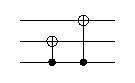
\includegraphics[scale=2]{Figures/circuits/vanillaCutsTemplate}};  
      \coordinate[below left=3.6mm and -6mm of circuit.west] (leftPoint1);
      \coordinate[below right=3.6mm and -6mm of circuit.east] (rightPoint1);
      \pic (cut1) {cut=leftPoint1/rightPoint1};
      \coordinate[above left=3.6mm and -6mm of circuit.west] (leftPoint2);
      \coordinate[above right=3.6mm and -6mm of circuit.east] (rightPoint2);
      \pic (cut2) {cut=leftPoint2/rightPoint2};
      \node[above left=4.5mm and -7mm of circuit.west, opacity=0.9] {\footnotesize \(A\)};
      \node[left=-7mm of circuit.west, opacity=0.9] {\footnotesize \(B\)};
      \node[below left=4.5mm and -7mm of circuit.west, opacity=0.9] {\footnotesize \(C\)};
      \node[right=-3mm of circuit.north west, font=\itshape] (text) {a)};
    \end{tikzpicture}
  };
  \node[above right=-28mm and 10mm of template] (hypergraph) {
    \begin{tikzpicture}
      \coordinate (O) at (0,0);
      \coordinate (A) at (90:10mm);
      \coordinate (B) at (210:10mm);
      \coordinate (C) at (330:10mm);
      \draw (O) -- (A);
      \draw (O) -- (B);
      \draw (O) -- (C);
      \node[circle, right=-2.5mm of A, fill=white, inner sep=0pt, minimum size=5mm] {\(A\)};
      \node[circle, right=-2.5mm of B, fill=white, inner sep=0pt, minimum size=5mm] {\(B\)};
      \node[circle, right=-2.5mm of C, fill=white, inner sep=0pt, minimum size=5mm] {\(C\)};
      \coordinate[above left=5.3mm and 9mm of O] (leftPoint);
      \coordinate[above right=5.3mm and 9mm of O] (rightPoint);
      \pic (cut) {cut=leftPoint/rightPoint};
      \coordinate (leftPoint2) at (270:10.5mm);
      \coordinate (rightPoint2) at (30:10.5mm);
      \pic (cut2) {cut=leftPoint2/rightPoint2};
      \coordinate (extraPoint) at (30:16mm);
      \pic (cut3) {cut=rightPoint2/extraPoint};
      \node[above left=0mm and 9mm of A, font=\itshape] (text) {b)};
    \end{tikzpicture}
  };
  \node[below right=2mm and -73mm of template] (distributed) {
    \begin{tikzpicture}[transform canvas={scale=0.65}]
      \node[inner sep=0pt] (circuit) {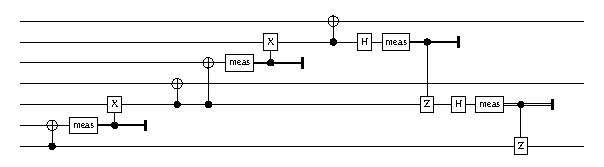
\includegraphics[scale=2]{Figures/circuits/vanillaCuts2}};
      \pic (e1) {ebit=e1/12.67mm/13mm};
      \pic (e2) {ebit=e2/33.84mm/13mm};
      \coordinate[above left=10.6mm and -6mm of circuit.west] (leftPoint);
      \coordinate[above right=10.6mm and -6mm of circuit.east] (rightPoint);
      \pic (cut) {cut=leftPoint/rightPoint};
      \coordinate[below left=10.6mm and -6mm of circuit.west] (leftPoint2);
      \coordinate[below right=10.6mm and -6mm of circuit.east] (rightPoint2);
      \pic (cut2) {cut=leftPoint2/rightPoint2};
      \node[above left=18.5mm and -7mm of circuit.west, opacity=0.9] {\footnotesize \(A\)};
      \node[left=-7mm of circuit.west, opacity=0.9] {\footnotesize \(B\)};
      \node[below left=18.5mm and -7mm of circuit.west, opacity=0.9] {\footnotesize \(C\)};
    \end{tikzpicture}
  };
  \node[right=-3mm of distributed.north west, font=\itshape] (text) {c)};
\end{tikzpicture}
\vspace*{38mm}
\caption{Same as in Figure~\ref{fig:vanillaCutsA}, but now there are two cuts, distributing the circuit across three QPUs.}
\label{fig:vanillaCutsC}
\end{figure}